\chapter{Introduction to linear regression}
\label{linRegrForTwoVar}

\index{linear regression|textbf}

Linear regression is a very powerful statistical technique. Many people have some familiarity with regression just from reading the news, where graphs with straight lines are overlaid on scatterplots. Linear models can be used for prediction or to evaluate whether there is a linear relationship between two numerical variables.

Figure~\ref{perfLinearModel} shows two variables whose relationship can be modeled perfectly with a straight line. The equation for the line is
\begin{eqnarray*}
y = 5 + 57.49x
\end{eqnarray*}
Imagine what a perfect linear relationship would mean: you would know the exact value of $y$ just by knowing the value of $x$. This is unrealistic in almost any natural process. For example, if we took family income $x$, this value would provide some useful information about how much financial support $y$ a college may offer a prospective student. However, there would still be variability in financial support, even when comparing students whose families have similar financial backgrounds.

\begin{figure}
   \centering
   \includegraphics[width=0.6\textwidth]{ch_regr_simple_linear/figures/perfLinearModel/perfLinearModel}
   \caption{Requests from twelve separate buyers were simultaneously placed with a trading company to purchase Target Corporation stock (ticker \texttt{TGT}, April 26th, 2012), and the total cost of the shares were reported. Because the cost is computed using a linear formula, the linear fit is perfect.}
   \label{perfLinearModel}
\end{figure}

Linear regression assumes that the relationship between two variables, $x$ and $y$, can be modeled by a straight line:
\begin{eqnarray}
y = \beta_0 + \beta_1x
\label{genLinModelWNoErrorTerm}
\end{eqnarray}
\marginpar[\raggedright\vspace{-10mm}

$\beta_0, \beta_1$\vspace{0.7mm}\\\footnotesize Linear model\\ parameters]{\raggedright\vspace{-10mm}

$\beta_0, \beta_1$\vspace{0.7mm}\\\footnotesize Linear model\\ parameters}where $\beta_0$ and $\beta_1$ represent two model parameters\index{parameter} ($\beta$ is the Greek letter \emph{beta}\index{Greek!beta@beta ($\beta$)}). (This use of $\beta$ has nothing to do with the $\beta$ we used to describe the probability of a Type~2 Error.) These parameters are estimated using data, and we write their point estimates as $b_0$ and $b_1$. When we use $x$ to predict $y$, we usually call $x$ the explanatory or \term{predictor} variable, and we call $y$ the response.

It is rare for all of the data to fall on a straight line, as seen in the three scatterplots in Figure~\ref{imperfLinearModel}. In each case, the data fall around a straight line, even if none of the observations fall exactly on the line. The first plot shows a relatively strong downward linear trend, where the remaining variability in the data around the line is minor relative to the strength of the relationship between $x$ and $y$. The second plot shows an upward trend that, while evident, is not as strong as the first. The last plot shows a very weak downward trend in the data, so slight we can hardly notice it. In each of these examples, we will have some uncertainty regarding our estimates of the model parameters, $\beta_0$ and $\beta_1$. For instance, we might wonder, should we move the line up or down a little, or should we tilt it more or less? As we move forward in this chapter, we will learn different criteria for line-fitting, and we will also learn about the uncertainty associated with estimates of model parameters.

\begin{figure}
   \centering
   \includegraphics[width=\textwidth]{ch_regr_simple_linear/figures/imperfLinearModel/imperfLinearModel}
   \caption{Three data sets where a linear model may be useful even though the data do not all fall exactly on the line.}
   \label{imperfLinearModel}
\end{figure}

We will also see examples in this chapter where fitting a straight line to the data, even if there is a clear relationship between the variables, is not helpful. One such case is shown in Figure~\ref{notGoodAtAllForALinearModel} where there is a very strong relationship between the variables even though the trend is not linear. We will discuss nonlinear trends in this chapter\MultipleRegressionChapter{ and the next}{}, but the details of fitting nonlinear models are saved for a later course.

\begin{figure}
   \centering
   \includegraphics[width=0.9\textwidth]{ch_regr_simple_linear/figures/notGoodAtAllForALinearModel/notGoodAtAllForALinearModel}
   \caption{A linear model is not useful in this nonlinear case. These data are from an introductory physics experiment.}
   \label{notGoodAtAllForALinearModel}
\end{figure}



\textA{\newpage}

%__________________
\section[Line fitting, residuals, and correlation]{Line fitting, residuals, and correlation \sectionvideohref{youtube-mPvtZhdPBhQ&list=PLkIselvEzpM63ikRfN41DNIhSgzboELOM}}
\label{lineFittingResidualsCorrelation}

It is helpful to think deeply about the line fitting process. In this section, we examine criteria for identifying a linear model and introduce a new statistic, \emph{correlation}.

\subsection{Beginning with straight lines}

\index{data!possum|(}

Scatterplots were introduced in Chapter~\ref{summarizingData} as a graphical technique to present two numerical variables simultaneously. Such plots permit the relationship between the variables to be examined with ease. Figure~\ref{scattHeadLTotalL} shows a scatterplot for the head length and total length of 104 brushtail possums from Australia. Each point represents a single possum from the data.

\begin{figure}
   \centering
   \includegraphics[width=0.85\textwidth]{ch_regr_simple_linear/figures/scattHeadLTotalL/scattHeadLTotalL}
   \caption{A scatterplot showing head length against total length for 104 brushtail possums. A point representing a possum with head length 94.1mm and total length 89cm is highlighted.}
   \label{scattHeadLTotalL}
\end{figure}

\setlength{\captionwidth}{0.9\mycaptionwidth}
\begin{figure}
   \centering
   \includegraphics[width=0.7\textwidth]{ch_regr_simple_linear/figures/possumPic/possumPic}
   \caption{The common brushtail possum of Australia.\vspace{-1mm} \\
   -----------------------------\vspace{-2mm}\\
   {\footnotesize Photo by Peter Firminger on Flickr: \oiRedirect{textbook-flickr_com_wollombi_58499575}{http://flic.kr/p/6aPTn} \oiRedirect{textbook-CC_BY_2}{CC~BY~2.0~license}.}\vspace{-8mm}}
   \label{possumPic}
\end{figure}
\setlength{\captionwidth}{\mycaptionwidth}

The head and total length variables are associated. Possums with an above average total length also tend to have above average head lengths. While the relationship is not perfectly linear, it could be helpful to partially explain the connection between these variables with a straight line.

\begin{figure}
   \centering
   \includegraphics[width=\textwidth]{ch_regr_simple_linear/figures/scattHeadLTotalLTube/scattHeadLTotalLTube}
   \caption{The figure on the left shows head length versus total length, and reveals that many of the points could be captured by a straight band. On the right, we see that a curved band is more appropriate in the scatterplot for \var{weight} and \var{mpgCity} from the \data{cars} data set.}
   \label{scattHeadLTotalLTube}
\end{figure}

Straight lines should only be used when the data appear to have a linear relationship, such as the case shown in the left panel of Figure~\ref{scattHeadLTotalLTube}. The right panel of Figure~\ref{scattHeadLTotalLTube} shows a case where a curved line would be more useful in understanding the relationship between the two variables.

\begin{caution}{Watch out for curved trends}
{We only consider models based on straight lines in this chapter. If data show a nonlinear trend, like that in the right panel of Figure~\ref{scattHeadLTotalLTube}, more advanced techniques should be used.\vspace{0.7mm}}
\end{caution}


\textA{\newpage}

\subsection{Fitting a line by eye}

We want to describe the relationship between the head length and total length variables in the possum data set using a line. In this example, we will use the total length as the predictor variable, $x$, to predict a possum's head length, $y$. We could fit the linear relationship by eye, as in Figure~\ref{scattHeadLTotalLLine}. The equation for this line is
\begin{eqnarray}
\hat{y} = 41 + 0.59x
\label{headLLinModTotalL}
\end{eqnarray}
We can use this line to discuss properties of possums. For instance, the equation predicts a possum with a total length of 80 cm will have a head length of
\begin{align*}
\hat{y} &= 41 + 0.59\times 80 \\
	&= 88.2 % mm
\end{align*}
A ``hat'' on $y$ is used to signify that this is an estimate. This estimate may be viewed as an average: the equation predicts that possums with a total length of 80 cm will have an average head length of 88.2 mm. Absent further information about an 80 cm possum, the prediction for head length that uses the average is a reasonable estimate.

\begin{figure}
   \centering
   \includegraphics[width=0.8\textwidth]{ch_regr_simple_linear/figures/scattHeadLTotalLLine/scattHeadLTotalLLine}
   \caption{A reasonable linear model was fit to represent the relationship between head length and total length.}
   \label{scattHeadLTotalLLine}
\end{figure}

\subsection{Residuals}

\index{residual|(}

\termsub{Residuals}{residual} are the leftover variation in the data after accounting for the model fit:
\begin{align*}
\text{Data} = \text{Fit} + \text{Residual}
\end{align*}
Each observation will have a residual. If an observation is above the regression line, then its residual, the vertical distance from the observation to the line, is positive. Observations below the line have negative residuals. One goal in picking the right linear model is for these residuals to be as small as possible.

Three observations are noted specially in Figure~\ref{scattHeadLTotalLLine}. The observation marked by an ``$\times$'' has a small, negative residual of about -1; the observation marked by ``$+$'' has a large residual of about +7; and the observation marked by ``$\triangle$'' has a moderate residual of about -4. The size of a residual is usually discussed in terms of its absolute value. For example, the residual for ``$\triangle$'' is larger than that of ``$\times$'' because $|-4|$ is larger than $|-1|$.

%\Comment{remove use of $e_i$ since students don't need that}

\begin{termBox}{\tBoxTitle{Residual: difference between observed and expected}
The residual of the $i^{th}$ observation $(x_i, y_i)$ is the difference of the observed response ($y_i$) and the response we would predict based on the model fit ($\hat{y}_i$):
\begin{eqnarray*}
\text{residual}_i = y_i - \hat{y}_i
\end{eqnarray*}
We typically identify $\hat{y}_i$ by plugging $x_i$ into the model.}
\end{termBox}

\begin{example}{The linear fit shown in Figure~\ref{scattHeadLTotalLLine} is given as $\hat{y} = 41 + 0.59x$. Based on this line, formally compute the residual of the observation $(77.0, 85.3)$. This observation is denoted by ``$\times$'' on the plot. Check it against the earlier visual estimate,~-1.}
We first compute the predicted value of point ``$\times$'' based on the model:
\begin{eqnarray*}
\hat{y}_{\times} = 41+0.59x_{\times} = 41+0.59\times 77.0 = 86.4
\end{eqnarray*}
Next we compute the difference of the actual head length and the predicted head length:
\begin{eqnarray*}
residual_{\times} = y_{\times} - \hat{y}_{\times} = 85.3 -  86.4 = -1.1
\end{eqnarray*}
This is very close to the visual estimate of -1.
\end{example}

\begin{exercise}
If a model underestimates an observation, will the residual be positive or negative? What about if it overestimates the observation?\footnote{If a model underestimates an observation, then the model estimate is below the actual. The residual, which is the actual observation value minus the model estimate, must then be positive. The opposite is true when the model overestimates the observation: the residual is negative.}
\end{exercise}

\begin{exercise}
Compute the residuals for the observations $(85.0, 98.6)$ (``$+$'' in the figure) and $(95.5, 94.0)$ (``$\triangle$'') using the linear relationship $\hat{y} = 41 + 0.59x$. \footnote{($+$) First compute the predicted value based on the model: $$\hat{y}_{+} = 41+0.59x_{+} = 41+0.59\times 85.0 = 91.15$$ Then the residual is given by $$residual_{+} = y_{+} - \hat{y}_{+} = 98.6-91.15=7.45$$This was close to the earlier estimate of 7.

($\triangle$) $\hat{y}_{\triangle} = 41+0.59x_{\triangle} = 97.3$. $residual_{\triangle} = y_{\triangle} - \hat{y}_{\triangle} = -3.3$, close to the estimate of -4.}
\end{exercise}

Residuals are helpful in evaluating how well a linear model fits a data set. We often display them in a \term{residual plot} such as the one shown in Figure~\ref{scattHeadLTotalLResidualPlot} for the regression line in Figure~\ref{scattHeadLTotalLLine}. The residuals are plotted at their original horizontal locations but with the vertical coordinate as the residual. For instance, the point $(85.0,98.6)_{+}$ had a residual of 7.45, so in the residual plot it is placed at $(85.0, 7.45)$. Creating a residual plot is sort of like tipping the scatterplot over so the regression line is horizontal. 

From the residual plot, we can better estimate the \term{standard deviation of the residuals}, often denoted by the letter $s$. %\footnote{This quanitity is also referred to as the standard deviation or standard error about the regression line and is sometimes denote $s_{RES}$, $s_e$ or $s_{\hat{y}}$. The formula is given by $s=\sqrt{\frac{\sum{(y_i-\hat{y})^2}}{n-2}}$, though it need not be memorized.}
The standard deviation of the residuals tells us the average size of the residuals.  As such, it is a measure of the average deviation between the $y$ values and the regression line.  In other words, it tells us the average prediction error using the linear model.

\begin{example}{Estimate the standard deviation of the residuals for predicting head length from total length using the regression line.  Also, interpret the quantity in context.}To estimate this graphically, we use the residual plot.  The approximate 68, 95 rule for standard deviations applies.  Approximately 2/3 of the points are within $\pm$ 2.5 and approximately 95\% of the points are within $\pm$ 5, so 2.5 is a good estimate for the standard deviation of the residuals.  On average, the prediction of head length is off by about 2.5 cm.

\index{data!possum|)}

\end{example}

\begin{termBox}{\tBoxTitle{Standard deviation of the residuals}
The standard deviation of the residuals, often denoted by the letter $s$, tells us the average error in the predictions using the regression model.  It can be estimated from a residual plot.}
\end{termBox}

\begin{figure}
   \centering
   \includegraphics[width=0.9\textwidth]{ch_regr_simple_linear/figures/scattHeadLTotalLResidualPlot/scattHeadLTotalLResidualPlot}
   \caption{Residual plot for the model in Figure~\ref{scattHeadLTotalLLine}.}
   \label{scattHeadLTotalLResidualPlot}
\end{figure}

\textA{\newpage}

\begin{example}{One purpose of residual plots is to identify characteristics or patterns still apparent in data after fitting a model. Figure~\ref{sampleLinesAndResPlots} shows three scatterplots with linear models in the first row and residual plots in the second row. Can you identify any patterns remaining in the residuals?}

\begin{figure}
   \centering
   \includegraphics[width=\textwidth]{ch_regr_simple_linear/figures/sampleLinesAndResPlots/sampleLinesAndResPlots}
   \caption{Sample data with their best fitting lines (top row) and their corresponding residual plots (bottom row).}
   \label{sampleLinesAndResPlots}
\end{figure}
In the first data set (first column), the residuals show no obvious patterns. The residuals appear to be scattered randomly around the dashed line that represents 0.

The second data set shows a pattern in the residuals. There is some curvature in the scatterplot, which is more obvious in the residual plot. We should not use a straight line to model these data. Instead, a more advanced technique should be used.

The last plot shows very little upwards trend, and the residuals also show no obvious patterns. It is reasonable to try to fit a linear model to the data. However, it is unclear whether there is statistically significant evidence that the slope parameter is different from zero. The point estimate of the slope parameter, labeled $b_1$, is not zero, but we might wonder if this could just be due to chance. We will address this sort of scenario in Section~\ref{inferenceForLinearRegression}.
\index{residual|)}
\end{example}


\textA{\newpage}

\subsection{Describing linear relationships with correlation}

\index{correlation|(}

\begin{termBox}{\tBoxTitle{Correlation coefficient, $r$, measures the strength of a linear relationship}
\termsub{Correlation}{correlation}, which always takes values between -1 and 1, describes the strength of the linear relationship between two variables. It can be strong, moderate, or~weak.}
\end{termBox}\marginpar[\raggedright\vspace{-11.5mm}

$r$\\\footnotesize correlation]{\raggedright\vspace{-11.5mm}

$r$\\\footnotesize correlation}

We can compute the correlation coefficient (or just correlation for short) using a formula, just as we did with the sample mean and standard deviation. However, this formula is rather complex,\footnote{Formally, we can compute the correlation for observations $(x_1, y_1)$, $(x_2, y_2)$, ..., $(x_n, y_n)$ using the formula
$r = \frac{1}{n-1}\sum_{i=1}^{n} \frac{x_i-\bar{x}}{s_x}\frac{y_i-\bar{y}}{s_y}$, 
where $\bar{x}$, $\bar{y}$, $s_x$, and $s_y$ are the sample means and standard deviations for each variable.} so we generally perform the calculations on a computer or calculator. Figure~\ref{posNegCorPlots} shows eight plots and their corresponding correlations. Only when the relationship is perfectly linear is the correlation either -1 or 1. If the relationship is strong and positive, the correlation will be near +1. If it is strong and negative, it will be near -1. If there is no apparent linear relationship between the variables, then the correlation will be near zero.

\begin{figure}
   \centering
   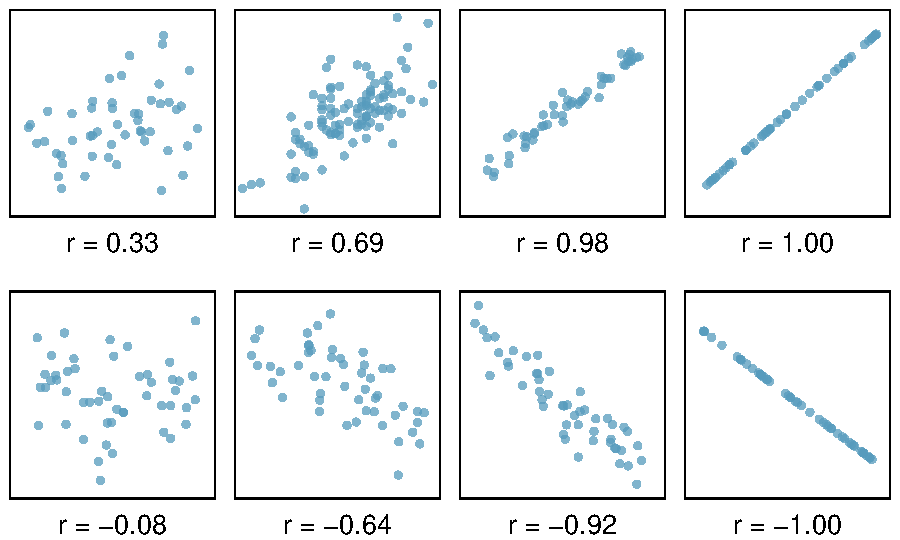
\includegraphics[width=0.95\textwidth]{ch_regr_simple_linear/figures/posNegCorPlots/posNegCorPlots}
   \caption{Sample scatterplots and their correlations. The first row shows variables with a positive relationship, represented by the trend up and to the right. The second row shows variables with a negative trend, where a large value in one variable is associated with a low value in the other.}
   \label{posNegCorPlots}
\end{figure}

The correlation is intended to quantify the strength of a linear trend. Nonlinear trends, even when strong, sometimes produce correlations that do not reflect the strength of the relationship; see three such examples in Figure~\ref{corForNonLinearPlots}.

\begin{figure}
   \centering
   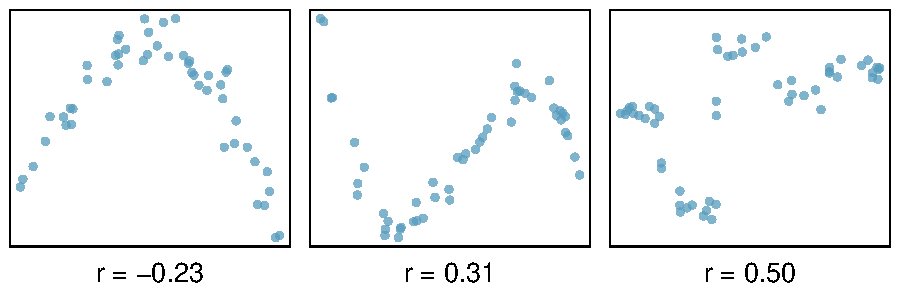
\includegraphics[width=0.96\textwidth]{ch_regr_simple_linear/figures/posNegCorPlots/corForNonLinearPlots}
   \caption{Sample scatterplots and their correlations. In each case, there is a strong relationship between the variables. However, the correlation is not very strong, and the relationship is not linear.}
   \label{corForNonLinearPlots}
\end{figure}

\begin{exercise}
It appears no straight line would fit any of the datasets represented in Figure~\ref{corForNonLinearPlots}. Try drawing nonlinear curves on each plot. Once you create a curve for each, describe what is important in your fit.\footnote{We'll leave it to you to draw the lines. In general, the lines you draw should be close to most points and reflect overall trends in the data.}
\index{correlation|)}
\end{exercise}

\begin{example}
{Take a look at Figure~\ref{scattHeadLTotalLLine} on page~\pageref{scattHeadLTotalLLine}.  How would this correlation change if head length were measured in cm rather than mm?  What if head length were measure in inches rather than mm?}Here, changing the units of $y$ corresponds to multiplying all the $y$ values by a certain number.  This would change the mean and the standard deviation of $y$, but it would not change the correlation.  To see this, imagine dividing every number on the vertical axes by 10.  The units of $y$ are now cm rather than mm, but the graph has remain exactly the same
\end{example}

\begin{termBox}{\tBoxTitle{Changing units of $x$ and $y$ does not affect $r$.}
The correlation between two variables should not be dependent upon the units in which the variables are recorded.  Adding a constant, subtracting a constant, or multiplying a \emph{positive} constant to all values of $x$ or $y$ does not affect the \mbox{correlation.}}
\end{termBox}


%__________________
\section[Fitting a line by least squares regression]{Fitting a line by least squares regression \sectionvideohref{youtube-z8DmwG2G4Qc&list=PLkIselvEzpM63ikRfN41DNIhSgzboELOM}}
\label{fittingALineByLSR}

\index{least squares regression|(}

Fitting linear models by eye is open to criticism since it is based on an individual preference. In this section, we use \emph{least squares regression} as a more rigorous approach.

This section considers family income and gift aid data from a random sample of fifty students in the 2011 freshman class of Elmhurst College in Illinois.\footnote{These data were sampled from a table of data for all freshman from the 2011 class at Elmhurst College that accompanied an article titled \emph{What Students Really Pay to Go to College} published online by \emph{The~Chronicle of Higher Education}: \oiRedirect{textbook-chronicle_elmhurst_article}{chronicle.com/article/What-Students-Really-Pay-to-Go/131435}} Gift aid is financial aid that does not need to be paid back, as opposed to a loan. A scatterplot of the data is shown in Figure~\ref{elmhurstScatterW2Lines} along with two linear fits. The lines follow a negative trend in the data; students who have higher family incomes tended to have lower gift aid from the university.

\begin{figure}
\centering
\includegraphics[width=0.75\textwidth]{ch_regr_simple_linear/figures/elmhurstPlots/elmhurstScatterW2Lines}
\caption{Gift aid and family income for a random sample of 50 freshman students from Elmhurst College. Two lines are fit to the data, the solid line being the \emph{least squares line}.}
\label{elmhurstScatterW2Lines}
\end{figure}

\begin{exercise}
Is the correlation positive or negative in Figure~\ref{elmhurstScatterW2Lines}?\footnote{Larger family incomes are associated with lower amounts of aid, so the correlation will be negative. Using a computer, the correlation can be computed: -0.499.}
\end{exercise}


\subsection{An objective measure for finding the best line}

We begin by thinking about what we mean by ``best''. Mathematically, we want a line that has small residuals. Perhaps our criterion could minimize the sum of the residual magnitudes:
\begin{eqnarray}
|y_1 - \hat{y}_1| + |y_2-\hat{y}_2| + \dots + |y_n-\hat{y}_n|
\label{sumOfAbsoluteValueOfResiduals}
\end{eqnarray}
which we could accomplish with a computer program. The resulting dashed line shown in Figure~\ref{elmhurstScatterW2Lines} demonstrates this fit can be quite reasonable. However, a more common practice is to choose the line that minimizes the sum of the squared residuals:
\begin{eqnarray}
(y_1 - \hat{y}_1)^2 + (y_2-\hat{y}_2)^2+ \dots + (y_n-\hat{y}_n)^2
\label{sumOfSquaresForResiduals}
\end{eqnarray}
The line that minimizes this \term{least squares criterion} is represented as the solid line in Figure~\ref{elmhurstScatterW2Lines}. This is commonly called the \term{least squares line}. The following are three possible reasons to choose Criterion~\eqref{sumOfSquaresForResiduals} over Criterion~\eqref{sumOfAbsoluteValueOfResiduals}:
\begin{enumerate}
\item It is the most commonly used method.
\item Computing the line based on Criterion~\eqref{sumOfSquaresForResiduals} is much easier by hand and in most statistical software.
\item In many applications, a residual twice as large as another residual is more than twice as bad. For example, being off by 4 is usually more than twice as bad as being off by 2. Squaring the residuals accounts for this discrepancy.
\end{enumerate}
The first two reasons are largely for tradition and convenience; the last reason explains why Criterion~\eqref{sumOfSquaresForResiduals} is typically most helpful.\footnote{There are applications where Criterion~\eqref{sumOfAbsoluteValueOfResiduals} may be more useful, and there are plenty of other criteria we might consider. However, this book only applies the least squares criterion.}

\subsection{Conditions for the least squares line}

When fitting a least squares line, we generally require
\begin{description}
\setlength{\itemsep}{0mm}
\item[Linearity.] The data should show a linear trend.  If there is a nonlinear trend (e.g. left panel of Figure~\ref{whatCanGoWrongWithLinearModel}), an advanced regression method from another book or later course should be applied.
\item[Nearly normal residuals.] Generally the residuals must be nearly normal.
When this condition is found to be unreasonable, it is usually because of outliers or concerns about influential points, which we  will discuss in greater depth in Section~\ref{typesOfOutliersInLinearRegression}. An example of non-normal residuals is shown in the second panel of Figure~\ref{whatCanGoWrongWithLinearModel}.
\item[Constant variability.] The variability of points around the least squares line remains roughly constant. An example of non-constant variability is shown in the third panel of Figure~\ref{whatCanGoWrongWithLinearModel}.
\end{description}

These conditions are best checked using a residual plot.  If a residual plot has no pattern, such as a U-shape or the presence of outliers or non-constant variability in the residuals, then the conditions above may be considered to be satisfied.

\begin{tipBox}{\tipBoxTitle{Use a residual plot to determine if a linear model is appropriate}
When a residual plot appears as a random cloud of points, a linear model is generally appropriate. If a residual plot has any type of pattern, a linear model is not appropriate.  
}
\end{tipBox} 



Be cautious about applying regression to data collected sequentially in what is called a \term{time series}. Such data may have an underlying structure that should be considered in a model and analysis.

\begin{figure}
\centering
\includegraphics[width=\textwidth]{ch_regr_simple_linear/figures/whatCanGoWrongWithLinearModel/whatCanGoWrongWithLinearModel}
\caption{Four examples showing when the methods in this chapter are insufficient to apply to the data. In the left panel, a straight line does not fit the data. In the second panel, there are outliers; two points on the left are relatively distant from the rest of the data, and one of these points is very far away from the line. In the third panel, the variability of the data around the line increases with larger values of $x$. In the last panel, a time series data set is shown, where successive observations are highly correlated.}
\label{whatCanGoWrongWithLinearModel}
\end{figure}

\begin{exercise}
Should we have concerns about applying least squares regression to the Elmhurst data in Figure~\ref{elmhurstScatterW2Lines}?\footnote{The trend appears to be linear, the data fall around the line with no obvious outliers, the variance is roughly constant. These are also not time series observations. Least squares regression can be applied to these data.}
\end{exercise}

\subsection{Finding the least squares line}
\label{findingTheLeastSquaresLineSection}

For the Elmhurst data, we could write the equation of the least squares regression line as
\begin{eqnarray*}
\widehat{aid} = \beta_0 + \beta_{1}\times family\_\hspace{0.3mm}income
\end{eqnarray*}
Here the equation is set up to predict gift aid based on a student's family income, which would be useful to students considering Elmhurst. These two values, $\beta_0$ and $\beta_1$, are the \emph{parameters} of the regression line.

As in Chapters~4-6, the parameters are estimated using observed data. In practice, this estimation is done using a computer in the same way that other estimates, like a sample mean, can be estimated using a computer or calculator. However, we can also find the parameter estimates by applying two properties of the least squares line:
\begin{itemize}
\item The slope of the least squares line can be estimated by
\begin{eqnarray}
b_1 = r\frac{s_y}{s_x}
\label{slopeOfLSRLine}
\end{eqnarray}
where $r$ is the correlation between the two variables, and $s_x$ and $s_y$ are the sample standard deviations of the explanatory variable %(variable on the horizontal axis) 
and response% (variable on the vertical axis)
, respectively.
\item If $\bar{x}$ is the mean of the horizontal variable (from the data) and $\bar{y}$ is the mean of the vertical variable, then the point $(\bar{x}, \bar{y})$ is on the least squares line. Plugging this point in for $x$ and $y$ in the least squares equation and solving for $b_0$ gives
\begin{align}
\bar{y} &= b_0 + b_1\bar{x}
&&b_0=\bar{y}-b_1\bar{x}
\label{interceptOfLSRLine}
\end{align}
When solving for the $y$-intercept, first find the slope, $b_1$, and plug the slope and the point $(\bar{x}, \bar{y})$ into the least squares equation.
\end{itemize}
\marginpar[\raggedright\vspace{0.5mm}

$b_0, b_1$\vspace{0.5mm}\\\footnotesize Sample\\estimates\\ of $\beta_0$, $\beta_1$]{\raggedright\vspace{0.5mm}

$b_0, b_1$\vspace{0.5mm}\\\footnotesize Sample\\estimates\\ of $\beta_0$, $\beta_1$}We use $b_0$ and $b_1$ to represent the point estimates of the parameters $\beta_0$ and $\beta_1$.

\begin{exercise}
Table~\ref{summaryStatsOfSATGPAData} shows the sample means for the family income and gift aid as \$101,800 and \$19,940, respectively. Plot the point $(101.8, 19.94)$ on Figure~\vref{elmhurstScatterW2Lines} to verify it falls on the least squares line (the solid line).\footnote{If you need help finding this location, draw a straight line up from the x-value of 100 (or thereabout). Then draw a horizontal line at 20 (or thereabout). These lines should intersect on the least squares line.}
\end{exercise}

\begin{table}[ht]
\centering
\begin{tabular}{l rr}
\hline
\vspace{-4mm} & & \\
\vspace{0.4mm}	&	\ \ family income, in \$1000s (``$x$'')	& \ \ gift aid, in \$1000s (``$y$'') \\
\hline
  \vspace{-3.9mm} & & \\
mean	& $\bar{x} = 101.8$		& $\bar{y} = 19.94$ \\
sd		& $s_x = 63.2$		& $s_y = 5.46$\vspace{0.4mm} \\
\hline
\vspace{-4mm}\ &\\
	& \multicolumn{2}{r}{$r=-0.499$} \\
\hline
\end{tabular}
\caption{Summary statistics for family income and gift aid.}
\label{summaryStatsOfSATGPAData}
\end{table}

\begin{exercise} \label{findingTheSlopeOfTheLSRLineForIncomeAndAid}
Using the summary statistics in Table~\ref{summaryStatsOfSATGPAData}, compute the slope and $y$-intercept for the regression line of gift aid against family income. Write the equation of the regression line.\footnote{Apply Equations~\eqref{slopeOfLSRLine} and~\eqref{interceptOfLSRLine} with the summary statistics from Table~\ref{summaryStatsOfSATGPAData} to compute the slope and $y$-intercept:
\begin{align*}
b_1 &= r\frac{s_y}{s_x} = (-0.499)\frac{5.46}{63.2} = -0.0431 \\
b_0 & = \bar{y} - b_1\bar{x} = 19.94 - (-0.0431)(101.8) = 24.3\\
\hat{y}&=24.3 - 0.0431x
	\qquad\text{or}\qquad
	\widehat{aid} = 24.3 - 0.0431 \text{family\_\hspace{0.3mm}income}
\end{align*}\vspace{-3mm}}
\end{exercise}

We mentioned earlier that a computer is usually used to compute the least squares line. A summary table based on computer output is shown in Table~\ref{rOutputForIncomeAidLSRLine} for the Elmhurst data. The first column of numbers provides estimates for ${b}_0$ and ${b}_1$, respectively. Compare these to the result from Guided Practice~\ref{findingTheSlopeOfTheLSRLineForIncomeAndAid}.

\begin{table}[ht]
\centering
\begin{tabular}{l rrrr}
  \hline
  \vspace{-3.7mm} & & & & \\
 & Estimate & Std. Error & t value & Pr($>$$|$t$|$) \\ 
  \hline
  \vspace{-3.6mm} & & & & \\
(Intercept) & 24.3193 & 1.2915 & 18.83 & 0.0000 \\ 
family\_\hspace{0.3mm}income & -0.0431 & 0.0108 & -3.98 & 0.0002 \\ 
  \hline
\end{tabular}
\caption{Summary of least squares fit for the Elmhurst data. Compare the parameter estimates in the first column to the results of Guided Practice~\ref{findingTheSlopeOfTheLSRLineForIncomeAndAid}.}
\label{rOutputForIncomeAidLSRLine}
\end{table}

\begin{example}{Examine the second, third, and fourth columns in Table~\ref{rOutputForIncomeAidLSRLine}. Can you guess what they represent?}
We'll describe the meaning of the columns using the second row, which corresponds to~$\beta_1$. The first column provides the point estimate for $\beta_1$, as we calculated in an earlier example: -0.0431. The second column is a standard error for this point estimate: 0.0108. The third column is a $T$ test statistic for the null hypothesis that $\beta_1 = 0$: $T=-3.98$. The last column is the p-value for the $T$ test statistic for the null hypothesis $\beta_1=0$ and a two-sided alternative hypothesis: 0.0002. We will get into more of these details in Section~\ref{inferenceForLinearRegression}.
\end{example}

\begin{example}{Suppose a high school senior is considering Elmhurst College. Can she simply use the linear equation that we have estimated to calculate her financial aid from the university?}
She may use it as an estimate, though some qualifiers on this approach are important. First, the data all come from one freshman class, and the way aid is determined by the university may change from year to year. Second, the equation will provide an imperfect estimate. While the linear equation is good at capturing the trend in the data, no individual student's aid will be perfectly predicted.
\index{least squares regression|)}
\end{example} 

\subsection{Interpreting regression line parameter estimates}

\index{least squares regression!interpreting parameters|(}

Interpreting parameters in a regression model is often one of the most important steps in the analysis.

\begin{example}{The slope and intercept estimates for the Elmhurst data are -0.0431 and 24.3. What do these numbers really mean?}
Interpreting the slope parameter is helpful in almost any application. For each additional \$1,000 of family income, we would expect a student to receive a net difference of $\$\text{1,000}\times (-0.0431) = -\$43.10$ in aid on average, i.e. \$43.10 \emph{less}. Note that a higher family income corresponds to less aid because the coefficient of family income is negative in the model. We must be cautious in this interpretation: while there is a real association, we cannot interpret a causal connection between the variables because these data are observational. That is, increasing a student's family income may not cause the student's aid to drop. (It would be reasonable to contact the college and ask if the relationship is causal, i.e. if Elmhurst College's aid decisions are partially based on students' family income.)

The estimated intercept $b_0=24.3$ (in \$1000s) describes the average aid if a student's family had no income. The meaning of the intercept is relevant to this application since the family income for some students at Elmhurst is \$0. In other applications, the intercept may have little or no practical value if there are no observations where $x$ is near zero.
\end{example}

\begin{termBox}{\tBoxTitle{Interpreting parameters in a linear model}
\vspace{-4mm}
\begin{itemize}
\setlength{\itemsep}{0mm}
\item The slope, $b_1$, describes the average increase or decrease in the $y$ variable if the explanatory variable $x$ is one unit larger. 
\item The y-intercept, $b_0$, describes the average or predicted outcome of $y$ if $x=0$.  The linear model must be valid all the way to $x=0$ for this to make sense, which in many applications is not the case.
\end{itemize}
}
\end{termBox}

\index{least squares regression!interpreting parameters|)}


\subsection{Extrapolation is treacherous}

\index{least squares regression!extrapolation|(}

{\em\small When those blizzards hit the East Coast this winter, it proved to my satisfaction that global warming was a fraud. That snow was freezing cold. But in an alarming trend, temperatures this spring have risen. Consider this: On February $6^{th}$ it was 10 degrees. Today it hit almost 80. At this rate, by August it will be 220 degrees. So clearly folks the climate debate rages on.\vspace{0.5mm}}

\noindent\hspace{\textwidth}\hspace{-40mm}Stephen Colbert

\noindent\hspace{\textwidth}\hspace{-40mm}April 6th, 2010 \footnote{\oiRedirect{textbook-colbert_extrapolation}{www.colbertnation.com/the-colbert-report-videos/269929}} \\

Linear models can be used to approximate the relationship between two variables. However, these models have real limitations. Linear regression is simply a modeling framework. The truth is almost always much more complex than our simple line. For example, we do not know how the data outside of our limited window will behave.

\begin{example}{Use the model $\widehat{aid} = 24.3 - 0.0431\times family\_\hspace{0.3mm}income$ to estimate the aid of another freshman student whose family had income of \$1 million.}
Recall that the units of family income are in \$1000s, so we want to calculate the aid for $family\_\hspace{0.3mm}income = 1000$:
\begin{align*}
\widehat{aid} &= 24.3 - 0.0431 \times family\_\hspace{0.3mm}income \\
\widehat{aid}&=24.3 - 0.431(1000) = -18.8
\end{align*}
The model predicts this student will have -\$18,800 in aid (!). Elmhurst College cannot (or at least does not) require any students to pay extra on top of tuition to attend.
\end{example}

Applying a model estimate to values outside of the realm of the original data is called \term{extrapolation}. Generally, a linear model is only an approximation of the real relationship between two variables. If we extrapolate, we are making an unreliable bet that the approximate linear relationship will be valid in places where it has not been analyzed.

\index{least squares regression!extrapolation|)}


\textA{\newpage}

\subsection{Using $R^2$ to describe the strength of a fit}

\index{least squares regression!R-squared ($R^2$)|(}

We evaluated the strength of the linear relationship between two variables earlier using the correlation coefficient, $r$. However, it is more common to explain the strength of a linear fit using $R^2$, called \termsub{R-squared}{least squares regression!R-squared ($R^2$)} or the \term{explained variance}. If provided with a linear model, we might like to describe how closely the data cluster around the linear fit.

%\Comment{TODO(David) Can you add a dashed horizontal line at ybar, and draw a dashed or dotted vertical line from one of the points to ybar and from that same point to yhat - to illustrate how to understand $r^2$?  See R$\_$sqGraphic.png on AP Statistics dropbox for an example.}

\begin{figure}
\centering
\includegraphics[width=0.75\textwidth]{ch_regr_simple_linear/figures/elmhurstPlots/elmhurstScatterWLSROnly}
\caption{Gift aid and family income for a random sample of 50 freshman students from Elmhurst College, shown with the least squares regression line.}
\label{elmhurstScatterWLSROnly}
\end{figure}

The $R^2$ of a linear model describes the amount of variation in the response that is explained by the least squares line. For example, consider the Elmhurst data, shown in Figure~\ref{elmhurstScatterWLSROnly}. The variance of the response variable, aid received, is $s_{aid}^2=29.8$. However, if we apply our least squares line, then this model reduces our uncertainty in predicting aid using a student's family income. The variability in the residuals describes how much variation remains after using the model: $s_{_{RES}}^2 = 22.4$.  In short, there was a reduction of
$$\frac{s_{aid}^2 - s_{_{RES}}^2}{s_{aid}^2}
	= \frac{29.8 - 22.4}{29.8} = \frac{7.5}{29.8}
	= 0.25$$
This is how we compute the $R^2$ value.\footnote{$R^2=1-\frac{s^2_{RES}}{s^2_y}$} It also corresponds to the square of the correlation coefficient, $r$, that~is, $R^2=r^2$.
\begin{align*}
R^2 &= 0.25 & r &= -0.499
\end{align*}

\begin{termBox}{\tBoxTitle{$R^2$ is the explained variance}
$R^2$ is always between 0 and 1, inclusive.  It tells us the proportion of variation in the $y$ values that is explained by a regression model.  The higher the value of $R^2$, the better the model ``explains" the reponse variable.
}
\end{termBox}

\begin{exercise}
If a linear model has a very strong negative relationship with a correlation of -0.97, how much of the variation in the response is explained by the explanatory variable?\footnote{About $R^2 = (-0.97)^2 = 0.94$ or 94\% of the variation in aid is explained by the linear model.}
\index{least squares regression!R-squared ($R^2$)|)}
\end{exercise}

\begin{exercise}
If a linear model has an $R^2$ or explained variance of 0.94, what is the correlation coefficient?\footnote{We take the square root of $R^2$ and get 0.97, but we must be careful, because $r$ could be 0.97 \emph{or} -0.97.  Without knowing the slope or seeing the scatterplot, we have no way of knowing if $r$ is positive or negative.}
\end{exercise}


\subsection{Calculator: linear correlation and regression}

\begin{termBox}{\tBoxTitle{\videohref{ti84_calculating_regression_summary_statistics} TI-84: finding $b_0$, $b_1$, $R^2$, and $r$ for a linear model}
Use \calctext{STAT}, \calctext{CALC}, \calctext{LinReg(a + bx)}.
\begin{enumerate}
\setlength{\itemsep}{0mm}
\item Choose \calctext{STAT}.
\item Right arrow to \calctext{CALC}.
\item Down arrow and choose \calctext{8:LinReg(a+bx)}.\vspace{-1.5mm}
  \begin{itemize}
  \item Caution: choosing \calctext{4:LinReg(ax+b)} will reverse $a$ and $b$.
  \end{itemize}
\item Let \calctext{Xlist} be \calctext{L1} and \calctext{Ylist} be \calctext{L2} (don't forget to enter the $x$ and $y$ values in L1 and \calctext{L2} before doing this calculation).  
\item Leave \calctext{FreqList} blank.
\item Leave \calctext{Store RegEQ} blank.
\item Choose Calculate and hit \calctext{ENTER}, which returns: \\[1mm]
\begin{tabular}{l l}
\calctext{a} & $b_0$, the y-intercept of the best fit line \\
\calctext{b} & $b_1$, the slope of the best fit line \\
$\calctextmath{r^2}$ & $R^2$, the explained variance \\
\calctext{r} & $r$, the correlation coefficient
\end{tabular}
\end{enumerate}
TI-83: Do steps 1-3, then enter the $x$ list and $y$ list separated by a comma, e.g. \calctext{LinReg(a+bx) L1, L2}, then hit \calctext{ENTER}.}
\end{termBox} 

\begin{tipBox}{\tipBoxTitle{What to do if $r^2$ and $r$ do not show up on a TI-83/84}
If $r^2$ and $r$ do now show up when doing \calctext{STAT}, \calctext{CALC}, \calctext{LinReg}, the \emph{diagnostics} must be turned on.  This only needs to be once and the diagnostics will remain on.
\begin{enumerate}
\setlength{\itemsep}{0mm}
\item Hit \calctext{2ND} \calctext{0} (i.e. \calctext{CATALOG}).
\item Scroll down until the arrow points at \calctext{DiagnosticOn}.
\item Hit \calctext{ENTER} and \calctext{ENTER} again. The screen should now say: \\[1mm]
\begin{tabular}{l l}
\calctext{DiagnosticOn} & \\
& \calctext{Done} \\
\end{tabular}
\end{enumerate}
}
\end{tipBox} 

\begin{tipBox}{\tipBoxTitle{What to do if a TI-83/84 returns: \calctext{ERR:}~\calctext{DIM MISMATCH}}
This error means that the lists, generally L1 and L2, do not have the same length.
\begin{enumerate}
\setlength{\itemsep}{0mm}
\item Choose \calctext{1:Quit}.
\item Choose \calctext{STAT},~\calctext{Edit} and make sure that the lists have the same number of entries.
\end{enumerate}
}
\end{tipBox} 

\begin{termBox}{\tBoxTitle[]{\videohref{casio_calculating_regression_summary_statistics} Casio fx-9750GII: finding $b_0$, $b_1$, $R^2$, and $r$ for a linear model}
\begin{enumerate}
\setlength{\itemsep}{0mm}
\item Navigate to \calctext{STAT} (\calcbutton{MENU} button, then hit the \calcbutton{2} button or select \calctext{STAT}).
\item Enter the $x$ and $y$ data into 2 separate lists, e.g. $x$ values in \calctext{List 1} and $y$ values in \calctext{List 2}. Observation ordering should be the same in the two lists. For example, if $(5, 4)$ is the second observation, then the second value in the $x$ list should be 5 and the second value in the $y$ list should be 4.
\item Navigate to \calctext{CALC} (\calcbutton{F2}) and then \calctext{SET} (\calcbutton{F6}) to set the regression context.\vspace{-1.5mm}
  \begin{itemize}
  \item To change the \calctext{2Var XList}, navigate to it, select \calctext{List} (\calcbutton{F1}), and enter the proper list number. Similarly, set \calctext{2Var YList} to the proper list.
  \end{itemize}
\item Hit \calcbutton{EXIT}.
\item Select \calctext{REG} (\calcbutton{F3}), \calctext{X} (\calcbutton{F1}), and \calctext{a+bx} (\calcbutton{F2}), which returns: \\[1mm]
\begin{tabular}{l l}
\calctext{a} & $b_0$, the y-intercept of the best fit line \\
\calctext{b} & $b_1$, the slope of the best fit line \\
\calctext{r} & $r$, the correlation coefficient \\
$\calctextmath{r^2}$ & $R^2$, the explained variance \\
\calctext{MSe} & Mean squared error, which you can ignore
\end{tabular} \\[1mm]
If you select \calctext{ax+b} (\calcbutton{F1}), the \calctext{a} and \calctext{b} meanings will be reversed.
\end{enumerate}}
\end{termBox} 

\begin{table}[h]
\centering
{\small
\begin{tabular}{ccc}
\hline
&\var{fed\_\hspace{0.3mm}spend} & \var{poverty} \\
\hline
  1 & 6.07 & 10.6  \\
  2 & 6.14 & 12.2  \\ 
  3 & 8.75 & 25.0  \\ 
  4  & 7.12 & 12.6  \\ 
  5 &5.13 & 13.4  \\ 
6 &  8.71 & 5.6\\ 
  7  & 6.70 & 7.9 \\ 
\hline
\end{tabular}}
\caption{Data for Guided Practice~\ref{subsetOfCountyForRegressionGP}.}
\label{subsetOfCountyForRegression}
\end{table}

\begin{exercise}\label{subsetOfCountyForRegressionGP}
Table~\ref{subsetOfCountyForRegression} contains values of federal spending per capita (rounded to the nearand percent of population in poverty for seven counties.  This is a subset of the \data{countyDF} data set from Chapter 1.  Use a calculator to find the equation of the least squares regression line for this partial data set.\footnote{$a=5.136$ and $b=1.056$, therefore $\hat{y}=5.136 + 1.056x$.}
\end{exercise}

\subsection{Categorical predictors with two levels (special topic)}
\label{categoricalPredictorsWithTwoLevels}

Categorical variables are also useful in predicting outcomes. Here we consider a categorical predictor with two levels (recall that a \emph{level} is the same as a \emph{category}). We'll consider Ebay auctions for a video game, \emph{Mario Kart} for the Nintendo Wii, where both the total price of the auction and the condition of the game were recorded.\footnote{These data were collected in Fall 2009 and may be found at \oiRedirect{textbook-openintro_org_stat}{openintro.org/stat}.} Here we want to predict total price based on game condition, which takes values \resp{used} and \resp{new}. A plot of the auction data is shown in Figure~\ref{marioKartNewUsed}.

\begin{figure}
\centering
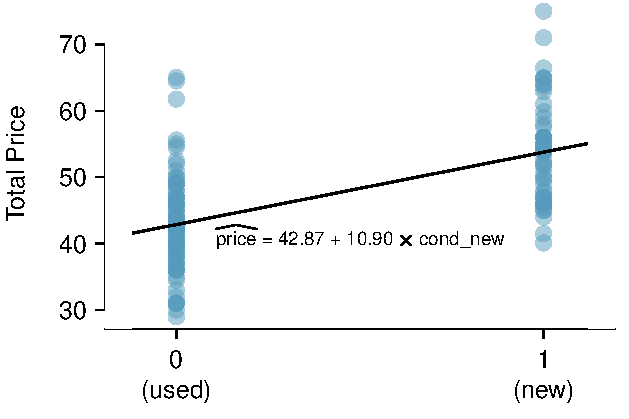
\includegraphics[width=0.65\textwidth]{ch_regr_simple_linear/figures/marioKartNewUsed/marioKartNewUsed}
\caption{Total auction prices for the video game \emph{Mario Kart}, divided into used ($x=0$) and new ($x=1$) condition games. The least squares regression line is also shown.}
\label{marioKartNewUsed}
\end{figure}

To incorporate the game condition variable into a regression equation, we must convert the categories into a numerical form. We will do so using an \term{indicator variable} called \var{cond\_\hspace{0.3mm}new}, which takes value 1 when the game is new and 0 when the game is used. Using this indicator variable, the linear model may be written as
\begin{align*}
\widehat{price} = \beta_0 + \beta_1 \times \text{\var{cond\_\hspace{0.3mm}new}}
\end{align*}
The fitted model is summarized in Table~\ref{marioKartNewUsedRegrSummary}, and the model with its parameter estimates is given as
\begin{align*}
\widehat{price} = 42.87 + 10.90 \times \text{\var{cond\_\hspace{0.3mm}new}}
\end{align*}
For categorical predictors with just two levels, the linearity assumption will always be satisfied. However, we must evaluate whether the residuals in each group are approximately normal and have approximately equal variance. As can be seen in Figure~\ref{marioKartNewUsed}, both of these conditions are reasonably satisfied by the auction data.

\begin{table}
\centering
\begin{tabular}{rrrrr}
  \hline
  \vspace{-3.7mm} & & & & \\
 & Estimate & Std. Error & t value & Pr($>$$|$t$|$) \\ 
  \hline
  \vspace{-3.6mm} & & & & \\
(Intercept) & 42.87 & 0.81 & 52.67 & 0.0000 \\ 
  cond\_\hspace{0.3mm}new & 10.90 & 1.26 & 8.66 & 0.0000 \\ 
   \hline
\end{tabular}
\caption{Least squares regression summary for the final auction price against the condition of the game.}
\label{marioKartNewUsedRegrSummary}
\end{table}

\begin{example}{Interpret the two parameters estimated in the model for the price of \emph{Mario Kart} in eBay auctions.}
The intercept is the estimated price when \var{cond\_\hspace{0.3mm}new} takes value 0, i.e. when the game is in used condition. That is, the average selling price of a used version of the game is \$42.87.

The slope indicates that, on average, new games sell for about \$10.90 more than used games.
\end{example}

\begin{tipBox}{\tipBoxTitle{Interpreting model estimates for categorical predictors.}
The estimated intercept is the value of the response variable for the first category (i.e. the category corresponding to an indicator value of 0). The estimated slope is the average change in the response variable between the two categories.}
\end{tipBox}



%__________________
\section[Types of outliers in linear regression]{Types of outliers in linear regression \sectionvideohref{youtube-jZEKAlo1E54&list=PLkIselvEzpM63ikRfN41DNIhSgzboELOM}}
\label{typesOfOutliersInLinearRegression}

In this section, we identify criteria for determining which outliers are important and influential.

Outliers in regression are observations that fall far from the ``cloud'' of points. These points are especially important because they can have a strong influence on the least squares line. 

\begin{example}{There are six plots shown in Figure~\ref{outlierPlots} along with the least squares line and residual plots. For each scatterplot and residual plot pair, identify any obvious outliers and note how they influence the least squares line. Recall that an outlier is any point that doesn't appear to belong with the vast majority of the other points.}\label{outlierPlotsExample}
\begin{itemize}
\item[(1)] There is one outlier far from the other points, though it only appears to slightly influence the line.
\item[(2)] There is one outlier on the right, though it is quite close to the least squares line, which suggests it wasn't very influential.
\item[(3)] There is one point far away from the cloud, and this outlier appears to pull the least squares line up on the right; examine how the line around the primary cloud doesn't appear to fit very well.
\item[(4)] There is a primary cloud and then a small secondary cloud of four outliers. The secondary cloud appears to be influencing the line somewhat strongly, making the least square line fit poorly almost everywhere. There might be an interesting explanation for the dual clouds, which is something that could be investigated.
\item[(5)] There is no obvious trend in the main cloud of points and the outlier on the right appears to largely control the slope of the least squares line.
\item[(6)] There is one outlier far from the cloud, however, it falls quite close to the least squares line and does not appear to be very influential.
\end{itemize}
\end{example}

\begin{figure}
\centering
\includegraphics[width=\textwidth]{ch_regr_simple_linear/figures/outlierPlots/outlierPlots}
\caption{Six plots, each with a least squares line and residual plot. All data sets have at least one outlier.}
\label{outlierPlots}
\end{figure}

Examine the residual plots in Figure~\ref{outlierPlots}. You will probably find that there is some trend in the main clouds of (3) and (4). In these cases, the outliers influenced the slope of the least squares lines. In (5), data with no clear trend were assigned a line with a large trend simply due to one outlier (!).
 
 \begin{termBox}{\tBoxTitle{Leverage}
Points that fall horizontally away from the center of the cloud tend to pull harder on the line, so we call them points with \term{high leverage}.}
\end{termBox}

Points that fall horizontally far from the line are points of high leverage; these points can strongly influence the slope of the least squares line. If one of these high leverage points does appear to actually invoke its influence on the slope of the line -- as in cases (3), (4), and (5) of Example~\ref{outlierPlotsExample} -- then we call it an \term{influential point}. Usually we can say a point is influential if, had we fitted the line without it, the influential point would have been unusually far from the least squares line.

It is tempting to remove outliers. Don't do this without a very good reason. Models that ignore exceptional (and interesting) cases often perform poorly. For instance, if a financial firm ignored the largest market swings -- the ``outliers'' --  they would soon go bankrupt by making poorly thought-out investments.

\begin{caution}{Don't ignore outliers when fitting a final model}
{If there are outliers in the data, they should not be removed or ignored without a~good reason. Whatever final model is fit to the data would not be very helpful if it ignores the most exceptional cases.}
\end{caution}

\begin{caution}{Outliers for a categorical predictor with two levels}
{Be cautious about using a categorical predictor when one of the levels has very few observations. When this happens, those few observations become influential points.}
\end{caution}



%__________________
\section[Inference for the slope of a regression line]{Inference for the slope of a regression line \sectionvideohref{youtube-depiT-hTaGA&list=PLkIselvEzpM63ikRfN41DNIhSgzboELOM}}
\label{inferenceForLinearRegression}

In this section we discuss uncertainty in the estimates of the slope and y-intercept for a regression line. Just as we identified standard errors for point estimates in previous chapters, we first discuss standard errors for these new estimates. However, in the case of regression, we will identify standard errors using statistical software.

%\Comment{rename with something more specific? hypothesis testing and ci for the slope?}
\subsection{Midterm elections and unemployment}

\index{data!midterm elections|(}

Elections for members of the United States House of Representatives occur every two years, coinciding every four years with the U.S. Presidential election. The set of House elections occurring during the middle of a Presidential term are called \indexthis{midterm elections}{midterm election}. In America's two-party system, one political theory suggests the higher the unemployment rate, the worse the President's party will do in the midterm elections.

To assess the validity of this claim, we can compile historical data and look for a connection. We consider every midterm election from 1898 to 2010, with the exception of those elections during the Great Depression. Figure~\ref{unemploymentAndChangeInHouse} shows these data and the least-squares regression line: \vspace{-2mm}
\begin{align*}
&\text{\% change in House seats for President's party}  \\
&\qquad\qquad= -6.71 - 1.00\times \text{(unemployment rate)}
\end{align*}
We consider the percent change in the number of seats of the President's party (e.g. percent change in the number of seats for Democrats in 2010) against the unemployment rate.

Examining the data, there are no clear deviations from linearity, the constant variance condition, or in the normality of residuals (though we don't examine a normal probability plot here). While the data are collected sequentially, a separate analysis was used to check for any apparent correlation between successive observations; no such correlation was found.

\begin{figure}
\centering
\includegraphics[width=0.95\textwidth]{ch_regr_simple_linear/figures/unemploymentAndChangeInHouse/unemploymentAndChangeInHouse}
\caption{The percent change in House seats for the President's party in each election from 1898 to 2010 plotted against the unemployment rate. The two points for the Great Depression have been removed, and a least squares regression line has been fit to the data.}
\label{unemploymentAndChangeInHouse}
\end{figure}

\begin{exercise}
The data for the Great Depression (1934 and 1938) were removed because the unemployment rate was 21\% and 18\%, respectively. Do you agree that they should be removed for this investigation? Why or why not?\footnote{We will provide two considerations. Each of these points would have very high leverage on any least-squares regression line, and years with such high unemployment may not help us understand what would happen in other years where the unemployment is only modestly high. On the other hand, these are exceptional cases, and we would be discarding important information if we exclude them from a final analysis.}
\end{exercise}

There is a negative slope in the line shown in Figure~\ref{unemploymentAndChangeInHouse}. However, this slope (and the y-intercept) are only estimates of the parameter values. We might wonder, is this convincing evidence that the ``true'' linear model has a negative slope? That is, do the data provide strong evidence that the political theory is accurate? We can frame this investigation into a one-sided statistical hypothesis test:
\begin{itemize}
\item[$H_0$:] $\beta_1 = 0$. The true linear model has slope zero.
\item[$H_A$:] $\beta_1 < 0$. The true linear model has a slope less than zero. The higher the unemployment, the greater the loss for the President's party in the House of Representatives.
\end{itemize}
We would reject $H_0$ in favor of $H_A$ if the data provide strong evidence that the true slope parameter is less than zero. To assess the hypotheses, we identify a standard error for the estimate, compute an appropriate test statistic, and identify the p-value.


\subsection{Understanding regression output from software}
\label{testStatisticForTheSlope}

Just like other point estimates we have seen before, we can compute a standard error and test statistic for $b_1$. We will generally label the test statistic using a $T$, since it follows the $t$-distribution.

\begin{tipBox}{\tipBoxTitle{Hypothesis tests on the slope of the regression line}
Use a $t$-test with $n - 2$ degrees of freedom when performing a hypothesis test on the slope of a regression line.}
\end{tipBox}


We will rely on statistical software to compute the standard error and leave the explanation of how this standard error is determined to a second or third statistics course. The table below shows software output for the least squares regression line in Figure~\ref{unemploymentAndChangeInHouse}. The row labeled \emph{unemp} represents the information for the slope, which is the coefficient of the unemployment variable.

\begin{tipBox}{\texttt{The regression equation is} \\

\texttt{Change = -6.7142 - 1.0010 unemp} \\

\texttt{Predictor \ \ \ \ \ Coef \ \ SE Coef \ \ \ \ \ \ T \ \ \ \ \ \ \ P} \\
\texttt{Constant \ \ \ -6.7142 \ \ \ 5.4567 \ \ -1.23 \ \ 0.2300} \\
\texttt{unemp \ \ \ \ \ \ -1.0010 \ \ \ 0.8717 \ \ -1.15 \ \ 0.2617} \\

\texttt{S = 9.624\ \ \ \ R-Sq = 0.03\% \ \ \ R-Sq(adj) = -3.7\%}}
\end{tipBox}
%\label{midtermElectionUnemploymentRRegressionOutput}

\begin{example}{What do the first and second columns of numbers in the regression summary represent?}
The entries in the first column represent the least squares estimates, $b_0$ and $b_1$, and the values in the second column correspond to the standard errors of each estimate.
\end{example}

We previously used a $T$ test statistic for hypothesis testing in the context of numerical data. Regression is very similar. In the hypotheses we consider, the null value for the slope is 0, so we can compute the test statistic using the $T$ score formula:
\begin{align*}
T = \frac{\text{estimate} - \text{null value}}{\text{SE}} = \frac{-1.0010 - 0}{0.8717} = -1.15
\end{align*}
We can look for the one-sided p-value -- shown in Figure~\ref{oneSidedTailForMidtermUnemploymentHT} -- using the probability table for the $t$-distribution in Appendix~\ref{tDistributionTable} on page~\pageref{tDistributionTable}.

\begin{figure}
\centering
\includegraphics[width=0.82\textwidth]{ch_regr_simple_linear/figures/oneSidedTailForMidtermUnemploymentHT/oneSidedTailForMidtermUnemploymentHT}
\caption{The distribution shown here is the sampling distribution for $b_1$, if the null hypothesis was true. The shaded tail represents the p-value for the hypothesis test evaluating whether there is convincing evidence that higher unemployment corresponds to a greater loss of House seats for the President's party during a midterm election.}
\label{oneSidedTailForMidtermUnemploymentHT}
\end{figure}

\begin{example}{In this example, the sample size $n=27$. Identify the degrees of freedom and p-value for the hypothesis test.}
The degrees of freedom for this test is $n-2$, or $df = 27-2 = 25$. Looking in the 25 degrees of freedom row in Appendix~\ref{tDistributionTable}, we see that the absolute value of the test statistic is smaller than any value listed, which means the tail area and therefore also the p-value is larger than 0.100 (one tail!). Because the p-value is so large, we fail to reject the null hypothesis. That is, the data do not provide convincing evidence that a higher unemployment rate has any correspondence with smaller or larger losses for the President's party in the House of Representatives in midterm elections.
\index{data!midterm elections|)}
\end{example}

We could have identified the $T$ test statistic from the software output of the regression model, shown in the \var{unemp} row and third column (t value). The entry in the \var{unemp} row and last column represents the p-value for the two-sided hypothesis test where the null value is zero. The corresponding one-sided test would have a p-value half of the listed value.

\begin{termBox}{\tBoxTitle{Inference for regression}
We usually rely on statistical software to identify point estimates and standard errors for parameters of a regression line. After verifying conditions hold for fitting a line, we can use the methods learned in Section~\ref{oneSampleMeansWithTDistribution} for the $t$-distribution to create confidence intervals for regression parameters or to evaluate hypothesis tests.}
\end{termBox}

\begin{caution}{Don't carelessly use the p-value from regression output}
{The last column in regression output often lists p-values for one particular hypothesis: a two-sided test where the null value is zero. If your test is one-sided and the point estimate is in the direction of $H_A$, then you can halve the software's p-value to get the one-tail area. If neither of these scenarios match your hypothesis test, be cautious about using the software output to obtain the p-value.}
\end{caution}

\begin{example}{Examine Figure~\vref{elmhurstScatterWLSROnly}, which relates the Elmhurst College aid and student family income. How sure are you that the slope is statistically significantly different from zero? That is, do you think a formal hypothesis test would reject the claim that the true slope of the line should be zero?} \label{overallAidIncomeInformalAssessmentOfRegressionLineSlope}
While the relationship between the variables is not perfect, there is an evident decreasing trend in the data. This suggests the hypothesis test will reject the null claim that the slope is zero.
\end{example}

Recall that $b_1=r\frac{s_y}{s_x}$.  If the slope of the true regression line is zero, the population correlation coefficient must also be zero.  The linear regression test for $\beta_1=0$ is equivalent, then, to a test for the population correlation coefficient $\rho=0$.

\begin{exercise}
The regression summary below shows statistical software output from fitting the least squares regression line shown in Figure~\ref{elmhurstScatterWLSROnly}. Use this output to formally evaluate the following hypotheses. $H_0$: The true slope of the regression line is zero. $H_A$: The true slope of the regression line is not zero.\footnote{We look in the second row corresponding to the family income variable. We see the point estimate of the slope of the line is -0.0431, the standard error of this estimate is 0.0108, and the $T$ test statistic is -3.98. The p-value corresponds exactly to the two-sided test we are interested in: 0.0002. The p-value is so small that we reject the null hypothesis and conclude that family income and financial aid at Elmhurst College for freshman entering in the year 2011 are negatively correlated and the true slope parameter is indeed less than 0, just as we believed in Example~\ref{overallAidIncomeInformalAssessmentOfRegressionLineSlope}.}
\end{exercise}

\begin{tipBox}{\texttt{The regression equation is} \\

\texttt{aid = 24.31933 - 0.04307 family\_income} \\

\texttt{Predictor \ \ \ \ \ \ \ Coef \ \ \ \ \ \ \ SE Coef \ \ T \ \ \ \ \ \ \ P} \\
\texttt{Constant \ \ \ \ \ \ \ \  24.31933 \ \ \ 1.29145 \ \ 18.831 \ \ < 2e-16} \\
\texttt{family\_income\ \ \ \ -0.04307 \ \ \ 0.01081 \ \ -3.985 \ \ 0.000229} \\

\texttt{S = 4.783\ \ \ \ R-Sq = 24.86\% \ \ \ R-Sq(adj) = 23.29\%}}
\end{tipBox}
%\label{rOutputForIncomeAidLSRLineInInferenceSection}

\begin{tipBox}{\tipBoxTitle{Always check assumptions}
If conditions for fitting the regression line do not hold, then the methods presented here should not be applied. The standard error or distribution assumption of the point estimate -- assumed to be normal when applying the $T$ test statistic -- may not be valid.}
\end{tipBox}


\subsection{Summarizing inference procedures for linear regression}

\begin{termBox}{\tBoxTitle[]{Hypothesis test for the slope of regression line}
\begin{enumerate}
\setlength{\itemsep}{0mm}
\item State the name of the test being used.\vspace{-1.5mm}
\begin{itemize}
\setlength{\itemsep}{0mm}
\item Linear regression $t$-test
\end{itemize}
\item Verify conditions.\vspace{-1.5mm}
\begin{itemize}
\setlength{\itemsep}{0mm}
\item The residual plot has no pattern.
\end{itemize}
\item Write the hypotheses in plain language.  No mathematical notation is needed for this test.\vspace{-1.5mm}
\begin{itemize}
\setlength{\itemsep}{0mm}
\item H$_0$: $\beta_1=0$, There is no significant linear relationship between [x] and~[y]. 
\item H$_A$: $\beta_1 \ne,\text{ or }<, \text{ or }>0$, There is a significant or significant negative or significant positive linear relationship between [x] and [y].  
\end{itemize}
\item Identify the significance level $\alpha$.
\item Calculate the test statistic and $df$: $T = \frac{\text{point estimate} - \text{null value}}{\text{SE of estimate}}$\vspace{-1.5mm}
\begin{itemize}
\setlength{\itemsep}{0mm}
\item The point estimate is $b_1$
\item $SE$ can be located on regression summary table next to value of $b_1$
\item $df = n-2$
\end{itemize}
\item Find the p-value, compare it to $\alpha$, and state whether to reject or not reject the null hypothesis.
\item Write the conclusion in the context of the question.
\end{enumerate}}
\end{termBox}

\textA{\newpage}

\begin{termBox}{\tBoxTitle[]{Constructing a confidence interval for the slope of regression line}
\begin{enumerate}
\setlength{\itemsep}{0mm}
\item State the name of the CI being used.\vspace{-1.5mm}
\begin{itemize}
\setlength{\itemsep}{0mm}
\item $t$-interval for slope of regression line
\end{itemize}
\item Verify conditions.\vspace{-1.5mm}
\begin{itemize}
\setlength{\itemsep}{0mm}
\item The residual plot has no pattern.
\end{itemize}
\item Plug in the numbers and write the interval in the form
$$\text{point estimate } \pm t^\star \times \text{SE of estimate}$$
\begin{itemize}
\setlength{\itemsep}{0mm}
\item The point estimate is $b_1$.
\item $df = n-2$
\item The critical value $t^*$ can be found on the $t$-table at row $df = n-2$
\item $SE$ can be located on regression summary table next to value of $b_1$
\end{itemize}
\item Evaluate the CI and write in the form ( $\_$ , $\_$ ).
\item Interpret the interval:  ``We are [XX]\% confident that this interval contains the true average increase in [y] for each additional [unit] of [x].
\item State the conclusion to the original question.
\end{enumerate}}
\end{termBox}


\textA{\newpage}

\subsection{Calculator: the linear regression $t$-test and $t$-interval}

When doing this type of inference, we generally make use of computer output that provides us with the necessary quantities: $b$ and $s_b$.  The calculator functions below require knowing all of the data and are, therefore, rarely used.  We describe them here for the sake of completion. 

\begin{termBox}{\tBoxTitle{\videohref{ti84_regression_t_test} TI-83/84: Linear regression $t$-test on $\beta_1$}
Use \calctext{STAT}, \calctext{TESTS}, \calctext{LinRegTTest}.
\begin{enumerate}
\setlength{\itemsep}{0mm}
\item Choose \calctext{STAT}.
\item Right arrow to \calctext{TESTS}.
\item Down arrow and choose \calctext{F:LinRegTest}. (On TI-83 it is \calctext{E:LinRegTTest}).
\item Let \calctext{Xlist} be \calctext{L1} and \calctext{Ylist} be \calctext{L2}. (Don't forget to enter the $x$ and $y$ values in \calctext{L1} and \calctext{L2} before doing this test.)
\item Let \calctext{Freq} be \calctext{1}.
\item Choose $\calctextmath{\ne}$, $\calctextmath{<}$, or $\calctextmath{>}$ to correspond to H$_A$.
\item Leave \calctext{RegEQ} blank.
\item Choose \calctext{Calculate} and hit \calcbutton{ENTER}, which returns: \\[1mm]
\begin{tabular}{ll l ll}
\calctext{t} & t statistic &\quad&
	\calctext{b} & $b_1$, slope of the line \\
\calctext{p} & p-value &&
	\calctext{s} & st.~dev.~of the residuals \\
\calctext{df} & degrees of freedom for the test &&
	$\calctextmath{r^2}$ & $R^2$, explained variance \\
\calctext{a} & $b_0$, y-intercept of the line &&
	\calctext{r} & $r$, correlation coefficient
\end{tabular}
\end{enumerate}
}
\end{termBox} 

\begin{termBox}{\tBoxTitle[]{\videohref{casio_regression_t_test} Casio fx-9750GII: Linear regression $t$-test on $\beta_1$}
\begin{enumerate}
\setlength{\itemsep}{0mm}
\item Navigate to \calctext{STAT} (\calcbutton{MENU} button, then hit the \calcbutton{2} button or select \calctext{STAT}).
\item Enter your data into 2 lists.
\item Select \calctext{TEST} (\calcbutton{F3}), \calctext{t} (\calcbutton{F2}), and \calctext{REG} (\calcbutton{F3}).
\item If needed, update the sidedness of the test and the \calctext{XList} and \calctext{YList} lists. The \calctext{Freq} should be set to \calctext{1}.
\item Hit \calcbutton{EXE}, which returns: \\[1mm]
\begin{tabular}{ll l ll}
\calctext{t} & t statistic &\quad&
	\calctext{b} & $b_1$, slope of the line \\
\calctext{p} & p-value &&
	\calctext{s} & st.~dev.~of the residuals \\
\calctext{df} & degrees of freedom for the test &&
	\calctext{r} & $r$, correlation coefficient \\
\calctext{a} & $b_0$, y-intercept of the line &&
	$\calctextmath{r^2}$ & $R^2$, explained variance
\end{tabular}
\end{enumerate}
}
\end{termBox} 

\textA{\newpage}

\begin{termBox}{\tBoxTitle{\videohref{ti84_regression_t_confint} TI-84: $t$-interval for $\beta_1$}
Use \calctext{STAT}, \calctext{TESTS}, \calctext{LinRegTInt}.
\begin{enumerate}
\setlength{\itemsep}{0mm}
\item Choose \calctext{STAT}.
\item Right arrow to \calctext{TESTS}.
\item Down arrow and choose \calctext{G:} \calctext{LinRegTest}.\vspace{-1.5mm}
  \begin{itemize}
  \item This test is not built into the TI-83.
  \end{itemize}
\item Let \calctext{Xlist} be \calctext{L1} and \calctext{Ylist} be \calctext{L2}. (Don't forget to enter the $x$ and $y$ values in \calctext{L1} and \calctext{L2} before doing this interval.)
\item Let \calctext{Freq} be \calctext{1}.
\item Enter the desired confidence level.
\item Leave \calctext{RegEQ} blank.
\item Choose \calctext{Calculate} and hit \calcbutton{ENTER}, which returns: \\[1mm]
\begin{tabular}{l l}
\calctext{(\underline{\ \ },\underline{\ \ })} & the confidence interval \\
\calctext{b} & $b_1$, the slope of best fit line of the sample data \\
\calctext{df} &degrees of freedom associated with this confidence interval \\
\calctext{s} & standard deviation of the residuals \\
\calctext{a} & $b_0$, the y-intercept of the best fit line of the sample data \\
$\calctextmath{r^2}$ & $R^2$, the explained variance \\
\calctext{r} & $r$, the correlation coefficient \\
\end{tabular}
\end{enumerate}
}
\end{termBox}



\section{Transformations for nonlinear data}

\subsection{Untransformed}

\begin{example}{Consider the scatterplot and residual plot in Figure~\ref{NeedsTransform-PreTransform}. The regression output is also provided.  Would a linear model be a good model for the data shown?}
First, we can note the $R^2$ value is fairly large.  However, this alone does not mean that the model is good.  Another model might be much better.  When assessing the appropriateness of a linear model, we should look at the residual plot.  The U pattern in the residual plot tells us the the original data is curved. If we inspect the two plots, we can see that for small and large values of $x$ we systematically underestimate $y$, whereas for middle values of $x$, we systematically overestimate $y$.  Because of the this, the model is not appropriate, and we should not carry out a linear regression $t$-test because the conditions for inference are not met.  However, we might be able to use a transformation to linearize the data.
\end{example}

\begin{figure}
   \centering
   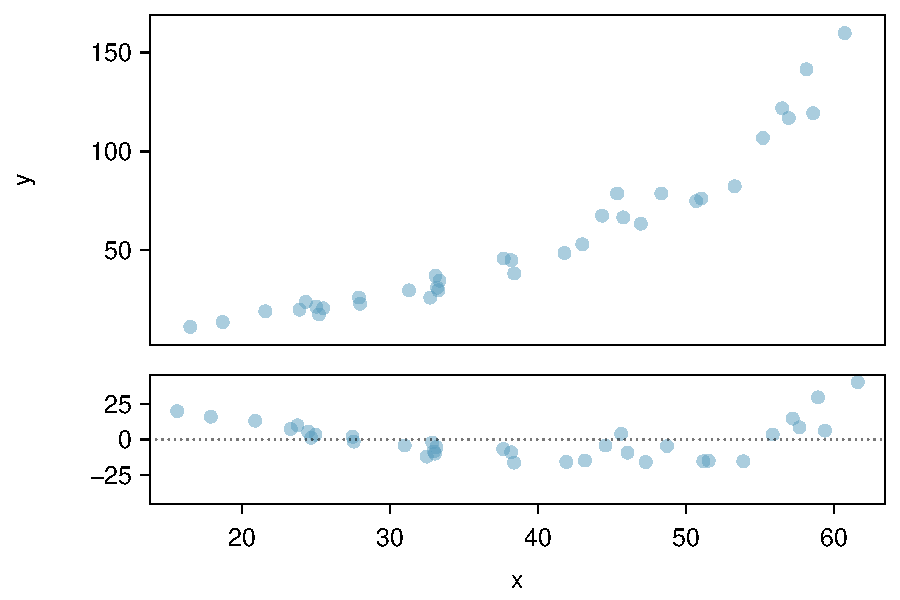
\includegraphics[width=0.7\textwidth]{ch_regr_simple_linear/figures/NeedsTransform/NeedsTransform-PreTransform}
   \caption{Variable $y$ is plotted against $x$. A nonlinear relationship is evident by the ``U'' shown in the residual plot. The curvature is also visible in the original plot.}
   \label{NeedsTransform-PreTransform}
\end{figure}

\textA{\newpage}

\begin{tipBox}{\texttt{The regression equation is} \\

\texttt{y = -52.3564 + 2.7842 x} \\

\texttt{Predictor \ \ \ \ \ \ Coef \ \ SE Coef \ \ \ \ \ \ \ \ T \ \ \ \ \ \ \ \ \ P} \\
\texttt{Constant \ \ \ -52.3564 \ \ \ 7.2757 \ \ \ -7.196 \ \ \ \ \ 3e-08} \\
\texttt{x \ \ \ \ \ \ \ \ \ \ \ \ 2.7842 \ \ \ 0.1768 \ \ \ 15.752 \ \ \ < 2e-16} \\

\texttt{S = 13.76\ \ \ \ R-Sq = 88.26\% \ \ \ R-Sq(adj) = 87.91\%}}
\end{tipBox}


\subsection{Transformed}

Regression analysis is easier to perform on linear data.  When data are nonlinear, we sometimes \term{transform} the data in a way that makes the resulting relationship linear.  The most common \term{transformation} is log (or ln) of the $y$ values. Sometimes we also apply a transformation to the $x$ values.  We generally use the residuals as a way to evaluate whether the transformed data are more linear. If so, we can say that a better model has been found.

\textA{\newpage}

\begin{example}{Using the regression output for the transformed data, write the new linear regression equation}
$\widehat{log(y)} = 1.723 +0.053 x$
\end{example}

\begin{figure}
   \centering
   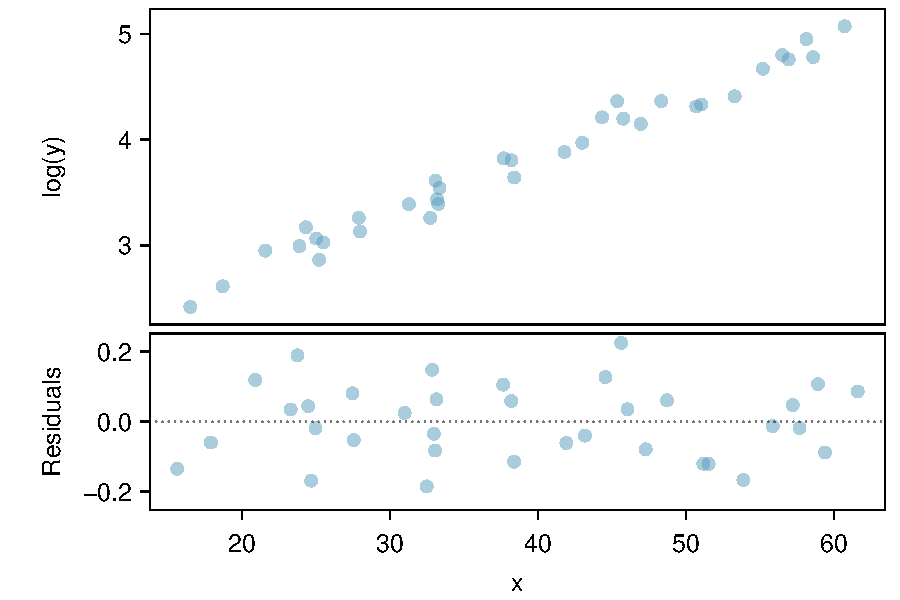
\includegraphics[width=0.7\textwidth]{ch_regr_simple_linear/figures/NeedsTransform/NeedsTransform-PostTransform}
   \caption{A plot of $\log(y)$ against $x$. The residuals don't show any evident patterns, which suggests the transformed data is well-fit by a linear model.}
   \label{NeedsTransform-PostTransform}
\end{figure}

\begin{tipBox}{\texttt{The regression equation is} \\

\texttt{log(y) = 1.722540 + 0.052985 x} \\

\texttt{Predictor \ \ \ \ \ \ \ \ Coef \ \ \ \ SE Coef \ \ \ \ \ \ \ T \ \ \ \ \ \ \ \ \ P} \\
\texttt{Constant \ \ \ \ \ 1.722540 \ \ \ 0.056731 \ \ \ 30.36 \ \ \ < 2e-16} \\
\texttt{x \ \ \ \ \ \ \ \ \ \ \ \ 0.052985 \ \ \ 0.001378 \ \ \ 38.45 \ \ \ < 2e-16} \\


\texttt{S = 0.1073\ \ \ \ R-Sq = 97.82\% \ \ \ R-Sq(adj) = 97.75\%}}
\end{tipBox}

\begin{exercise}Which of the following statements are true?  There may be more than one.\footnote{Part~(a) is \emph{false} since there is a nonlinear (curved) trend in the data. Part~(b) is true. Since the transformed data shows a stronger linear trend, it is a better fit, i.e. Part~(c) is \emph{false}, and Part~(d) is true.}
\begin{enumerate}[(a)]
\item There is an apparent linear relationship between $x$ and $y$.
\item There is an apparent linear relationship between $x$ and $\widehat{log(y)}$.
\item The model provided by Regression I ($\hat{y} = -52.3564 + 2.7842 x$) yields a better~fit.
\item The model provided by Regression II ($\widehat{log(y)} = 1.723 +0.053 x$) yields a better~fit.
\end{enumerate}
\end{exercise}
